\section{Voltage Control}
\label{sec:voltagecontrol}

There are two common approaches for controlling a simple DC motor, current control and voltage control~\cite{motorControl}.
%	This really should be cited.
Since motor torque is directly related to current, the output of a current controller corresponds to the desired motor torque~\cite{current}.
Similarly, since motor speed is directly related to its armature voltage, the output of a voltage controller corresponds to the desired motor speed~\cite{voltage}.
The PID controller used for this project is designed to be a voltage controller.
As such, its output is the desired voltage across the armature or alternatively the desired motor speed.

It is important to note that the PWM amplifier used in this project (either software PWM or the original hardware PWM) is NOT in inherently a voltage amplifier but an open loop power amplifier.
Its input signal controls the on-off power-supply duty cycle seen by the load each period. 
For a purely resistive load, a PWM amplifier may be used as a voltage amplifier.
The motor however, produces back EMF that is directly proportional to the speed of the armature.
In other words, the load characteristics change based on motor speed.
As such, there is no direct correlation between the PWM amplifier  input voltage and its output voltage when connected to a motor.
Without compensating for back EMF, the lookup table technique used by most other groups is valid only for the motor speed and load for which it was designed. 
The general approach is naive, highly inaccurate, and unsuitable for a position control system.

The Simulink block diagram used to condition the controller output signal and compensate for limitations of the PWM amplification technique may be seen in Figure \ref{fig:simulinkvoltagecontrol}.
In addition to back EMF compensation, simple error compensation is also used.
The actual armature voltage is measured, compared to the desired voltage and the resulting error signal added.
A final form of compensation, simple feed forward, is also introduced.
It was added to correct for a consistent offset observed in the measured motor voltage signal.
A demonstration of voltage control performance may be seen in Figure \ref{fig:backemf}. 
The measured voltage tracks the input voltage very well, showing the excellent degree of control which can be obtained using a software based solution.
It should be noted that over the course of the test, there was significant load variation, manually applied to the motor shaft, with very little impact on its speed.

%The motor in our system produces back EMF that is directly proportional to the speed of the armature.
%The current through the motor is controlled by the difference between the battery voltage and the back EMF. 

%The Voltage Control plot below shows the results of measuring the motor voltage across the terminals along side the controller input voltage, which has had the effects of back emf eliminated from the signal.  
%What is prominent is how closely the measured voltage tracks the input voltage from the controller, showing the excellent degree of voltage control obtained using a software based solution.


\begin{figure}[htp]
    \centering
    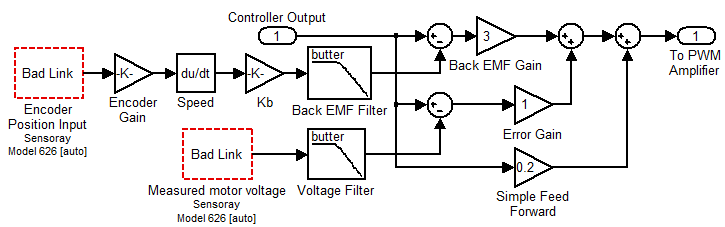
\includegraphics[scale=0.7]{images/VoltageControl.PNG}
    \caption{Voltage Control}
    \label{fig:simulinkvoltagecontrol}
\end{figure}

\begin{figure}[htp]
    \centering
    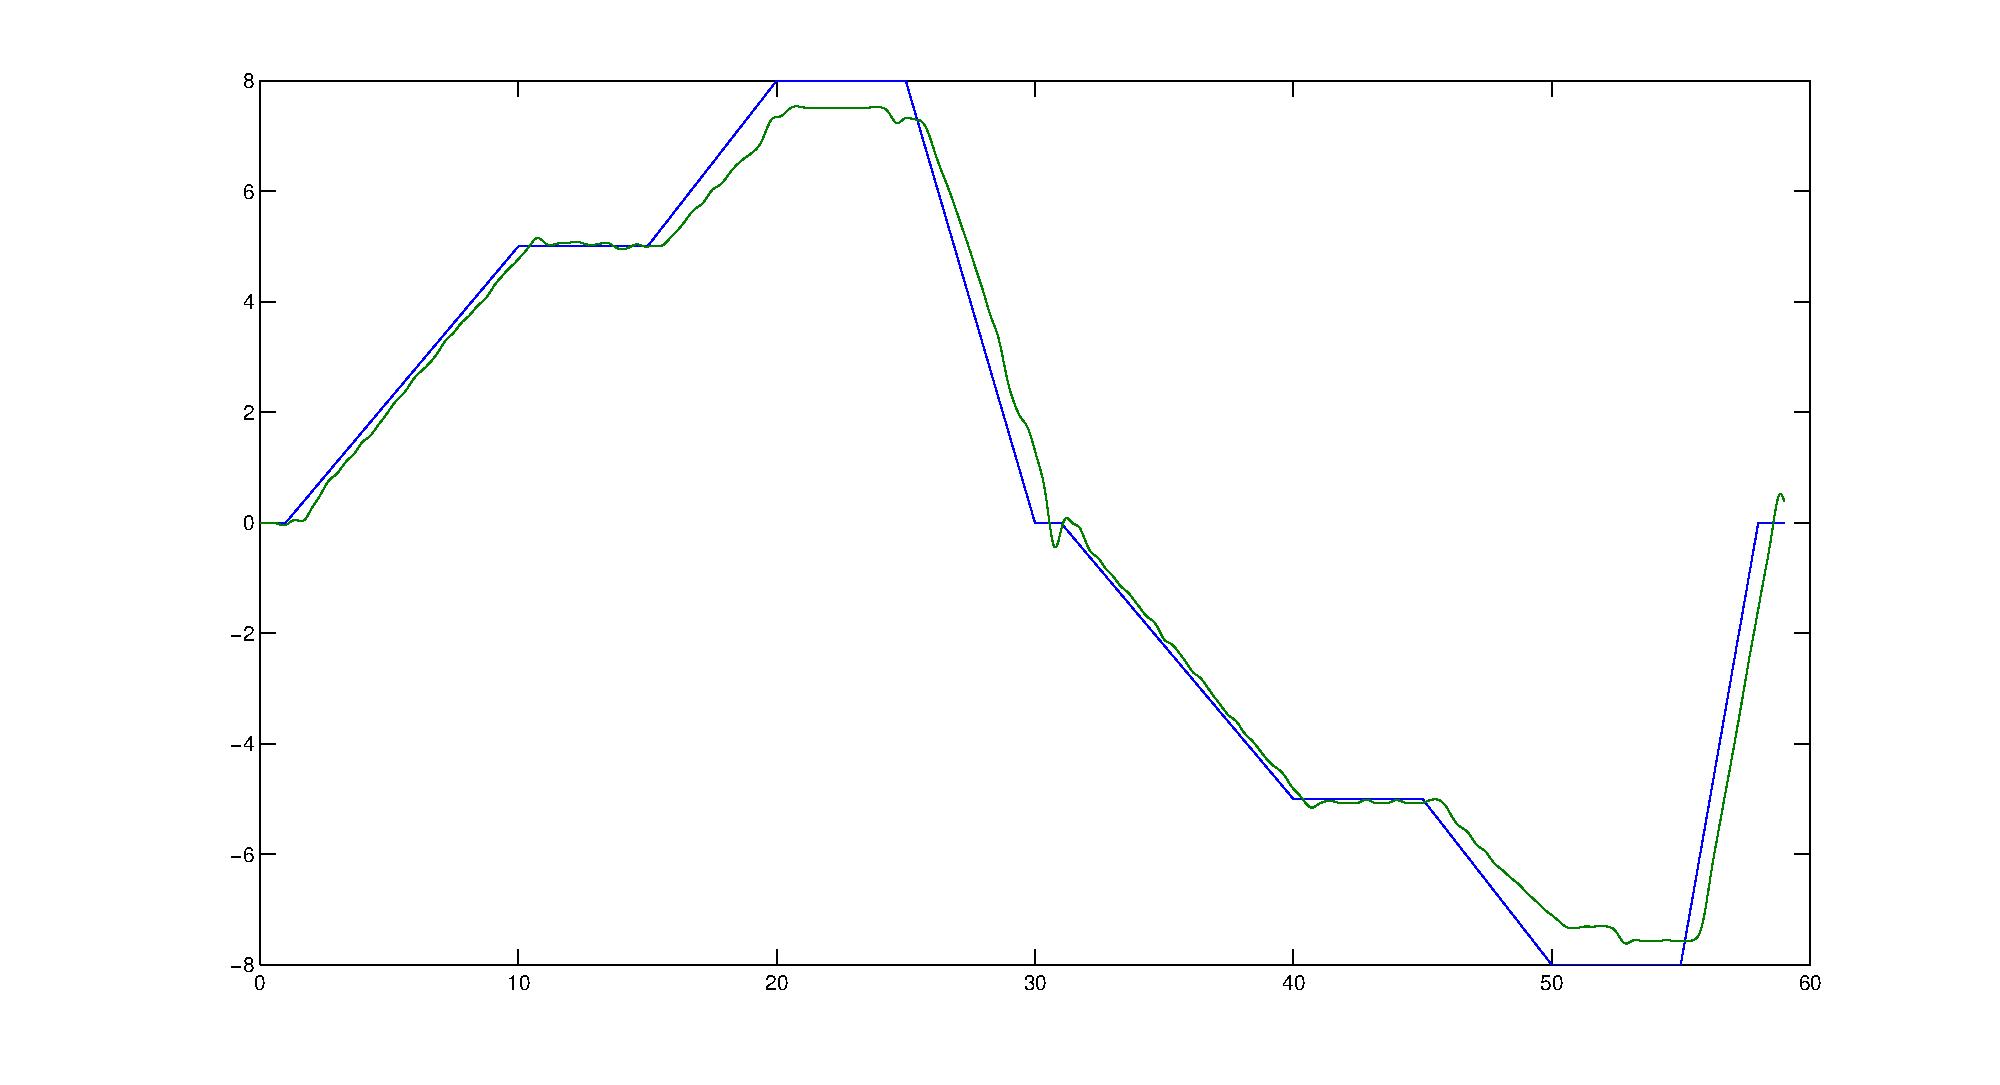
\includegraphics[width=.9\textwidth]{images/BackEMFControl.pdf}
    \caption{Voltage Control With Back EMF Compensation}
    \label{fig:backemf}
\end{figure}
